\documentclass{beamer}
\usepackage{relsize}
\usepackage{color}

\usepackage{listings}
\usetheme{CambridgeUS}
%\usepackage{beamerthemesplit} % new
\usepackage{enumitem}
\usepackage{amsmath}                    % See geometry.pdf to learn the layout options.
\usepackage{amsthm}                   % See geometry.pdf to learn the layout options. There
\usepackage{amssymb}                    % See geometry.pdf to learn the layout options.
\usepackage[utf8]{inputenc}
\usepackage{graphicx}
\usepackage[english,bulgarian]{babel}

\usetheme{CambridgeUS}
\usecolortheme{crane}

\lstset{language=C++,
                basicstyle=\ttfamily,
                keywordstyle=\color{blue}\ttfamily,
                stringstyle=\color{red}\ttfamily,
                commentstyle=\color{green}\ttfamily,
                morecomment=[l][\color{magenta}]{\#}
}

\newtheorem{mydef}{Дефиниция}[section]
\newtheorem{lem}{Лема}[section]
\newtheorem{thm}{Твърдение}[section]

\DeclareMathOperator{\restrict}{\upharpoonright}

\setitemize{label=\usebeamerfont*{itemize item}%
  \usebeamercolor[fg]{itemize item}
  \usebeamertemplate{itemize item}}

\setbeamercovered{transparent}



\begin{document}
\title[Увод в курса]{Въведение във функционалното програмиране}
\frame{\titlepage}

\section{Увод}
\subsection{Императивно vs. функционално програмиране}

\frame{\frametitle{Von Neumann архитектура}

\begin{figure}
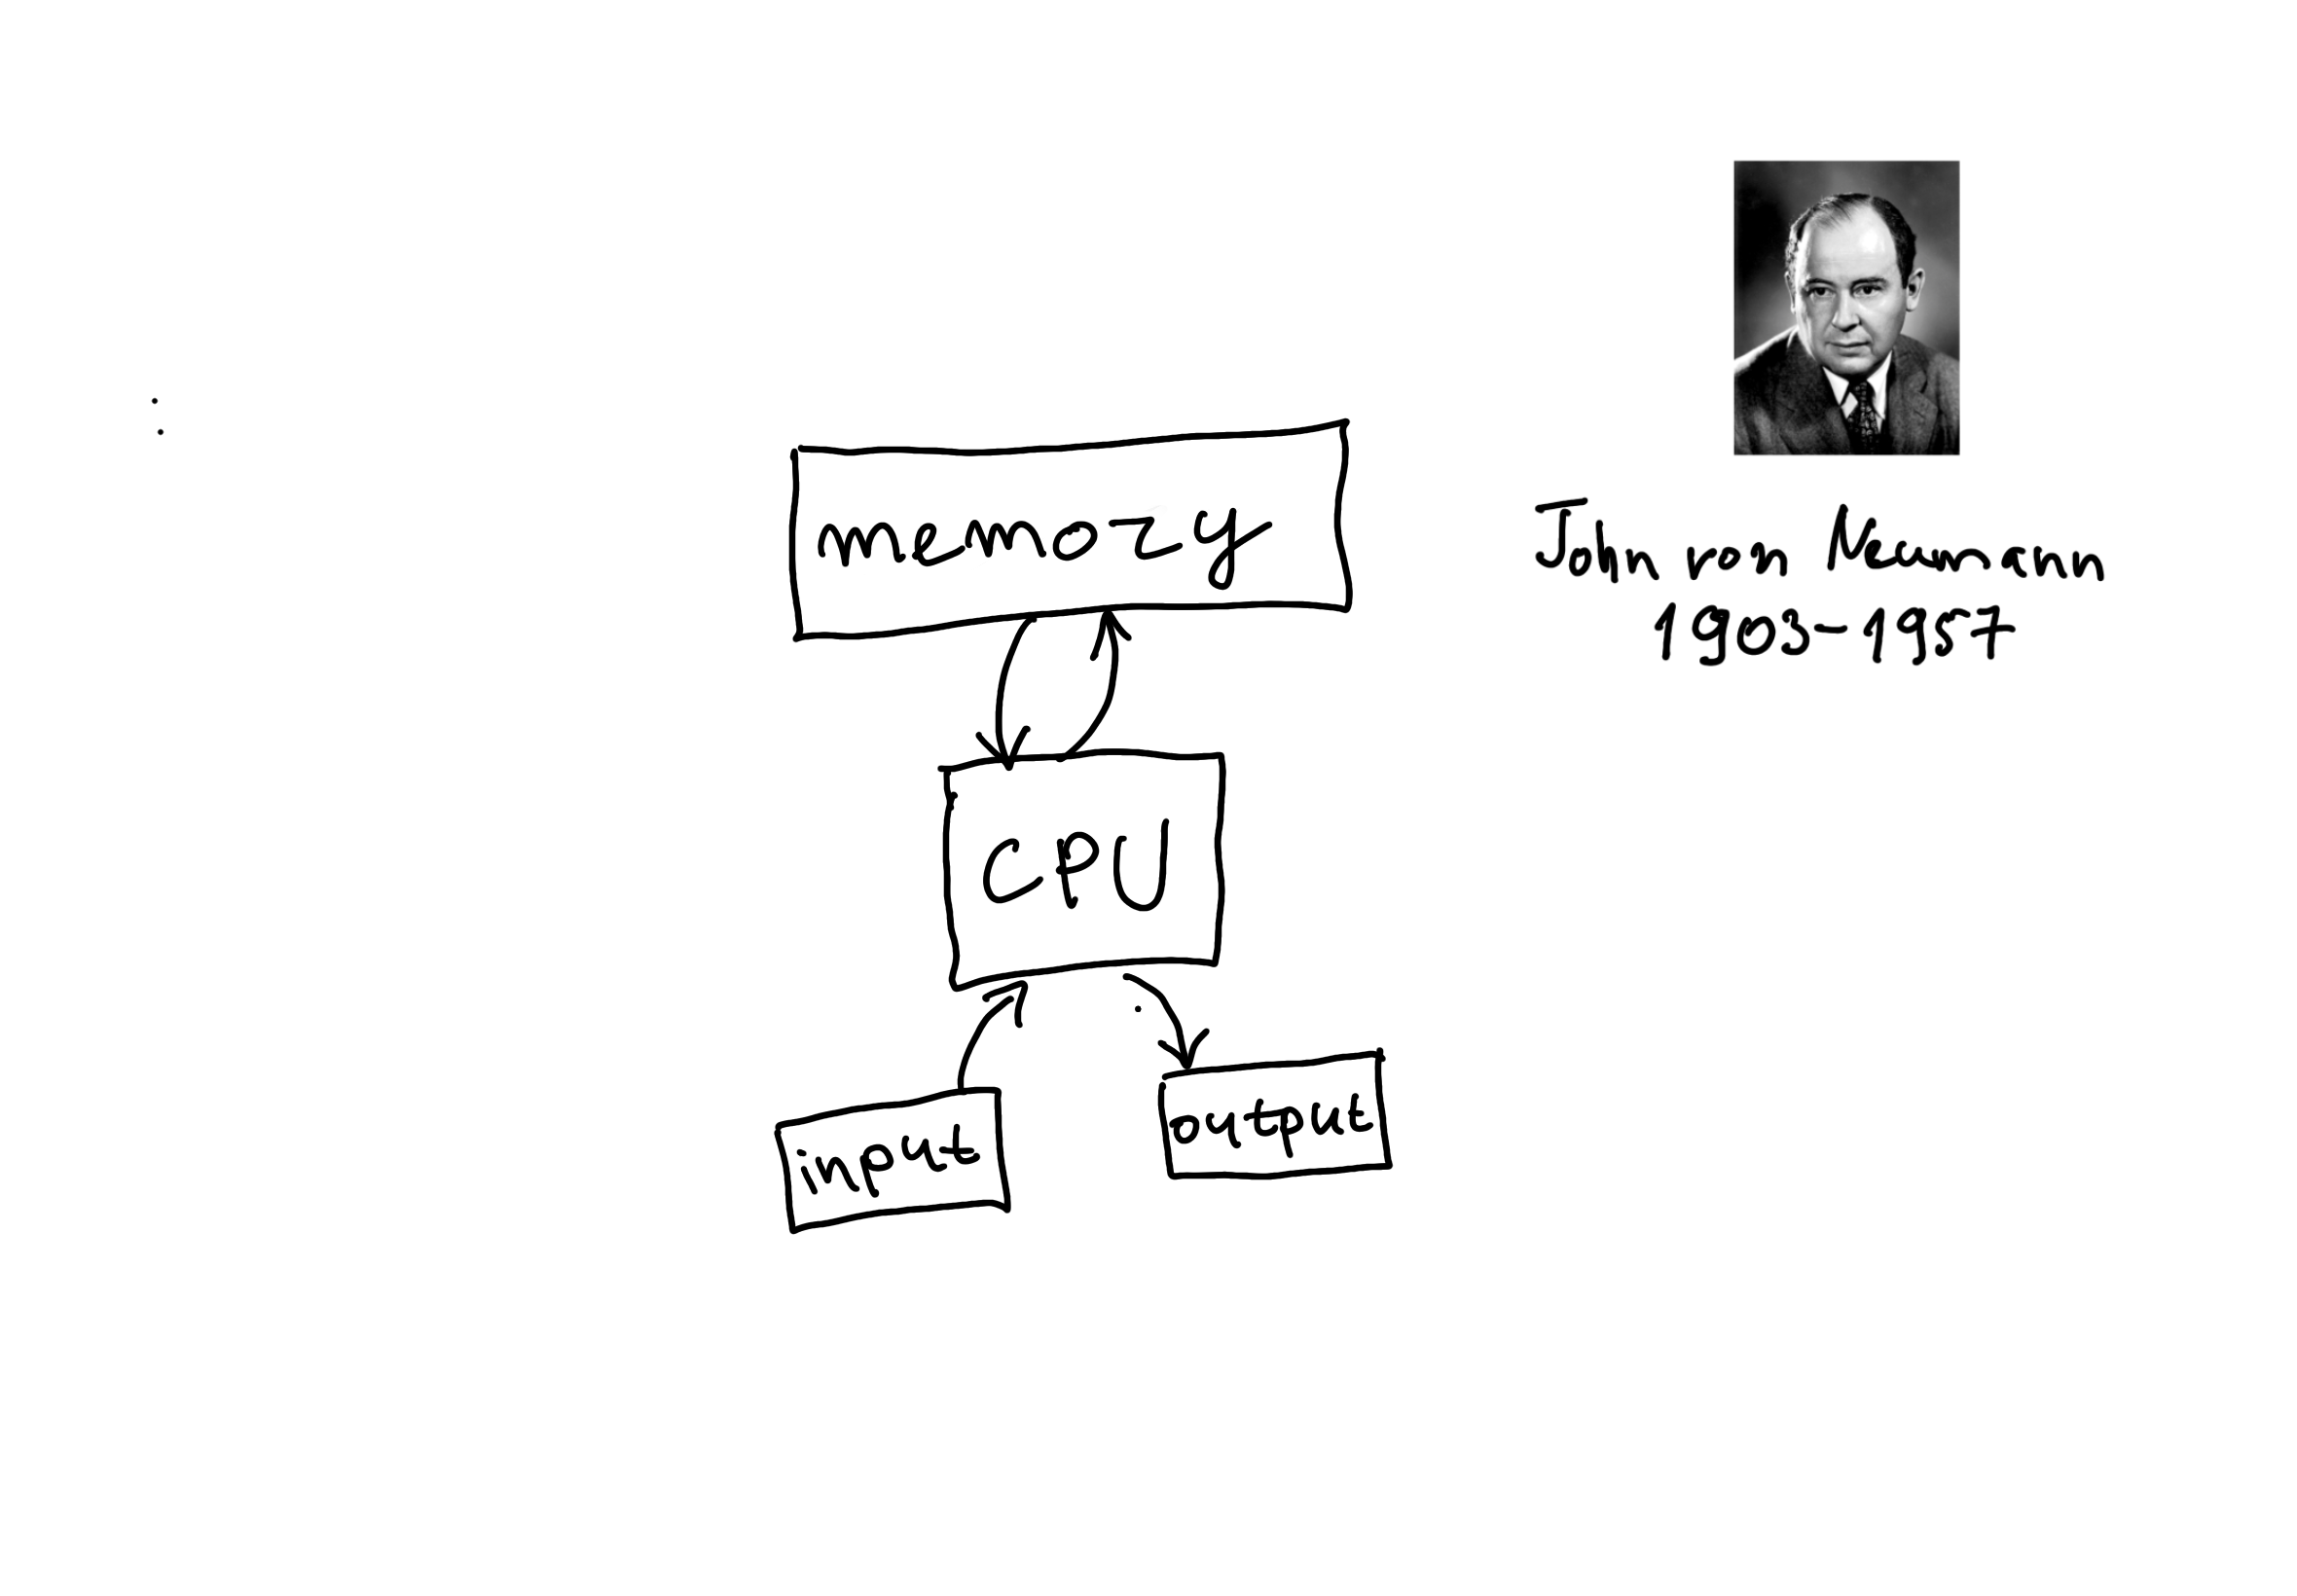
\includegraphics[width=12cm]{images/von-neumann}
\end{figure}

}

\frame{\frametitle{Императивен стил}

\begin{figure}
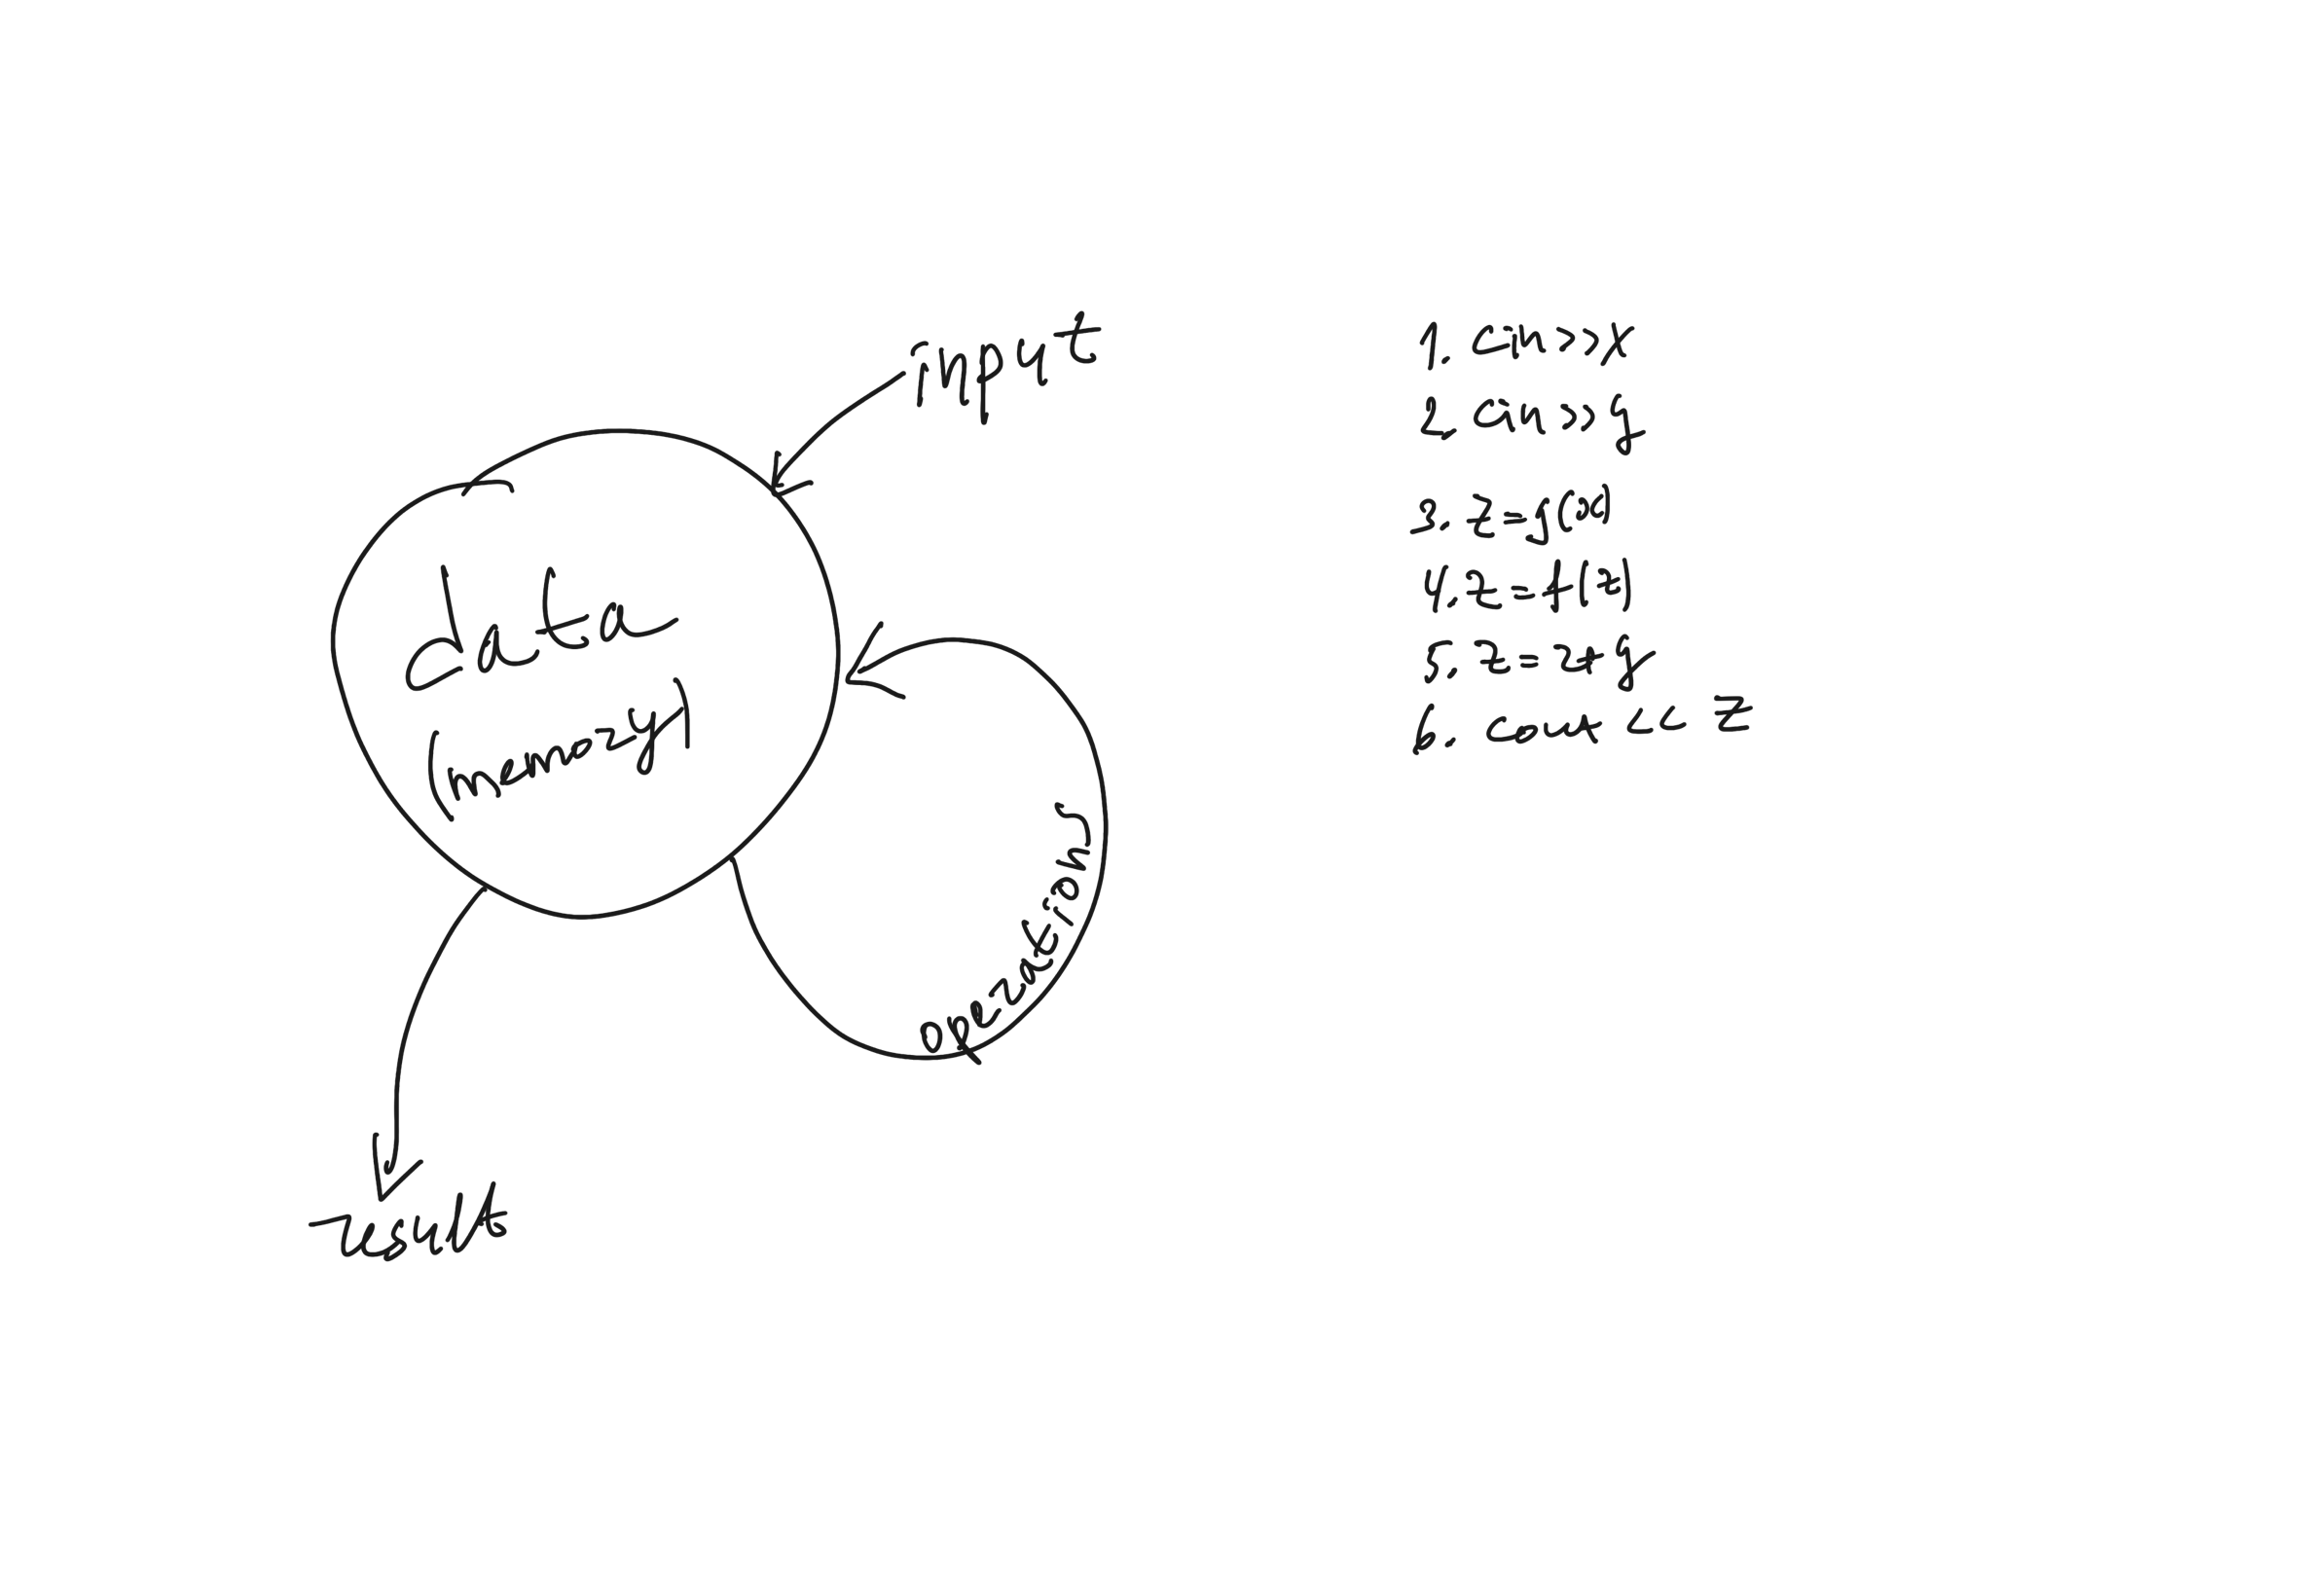
\includegraphics[width=12cm]{images/data-operations}
\end{figure}

}


\frame{\frametitle{Функционален стил}

\begin{figure}
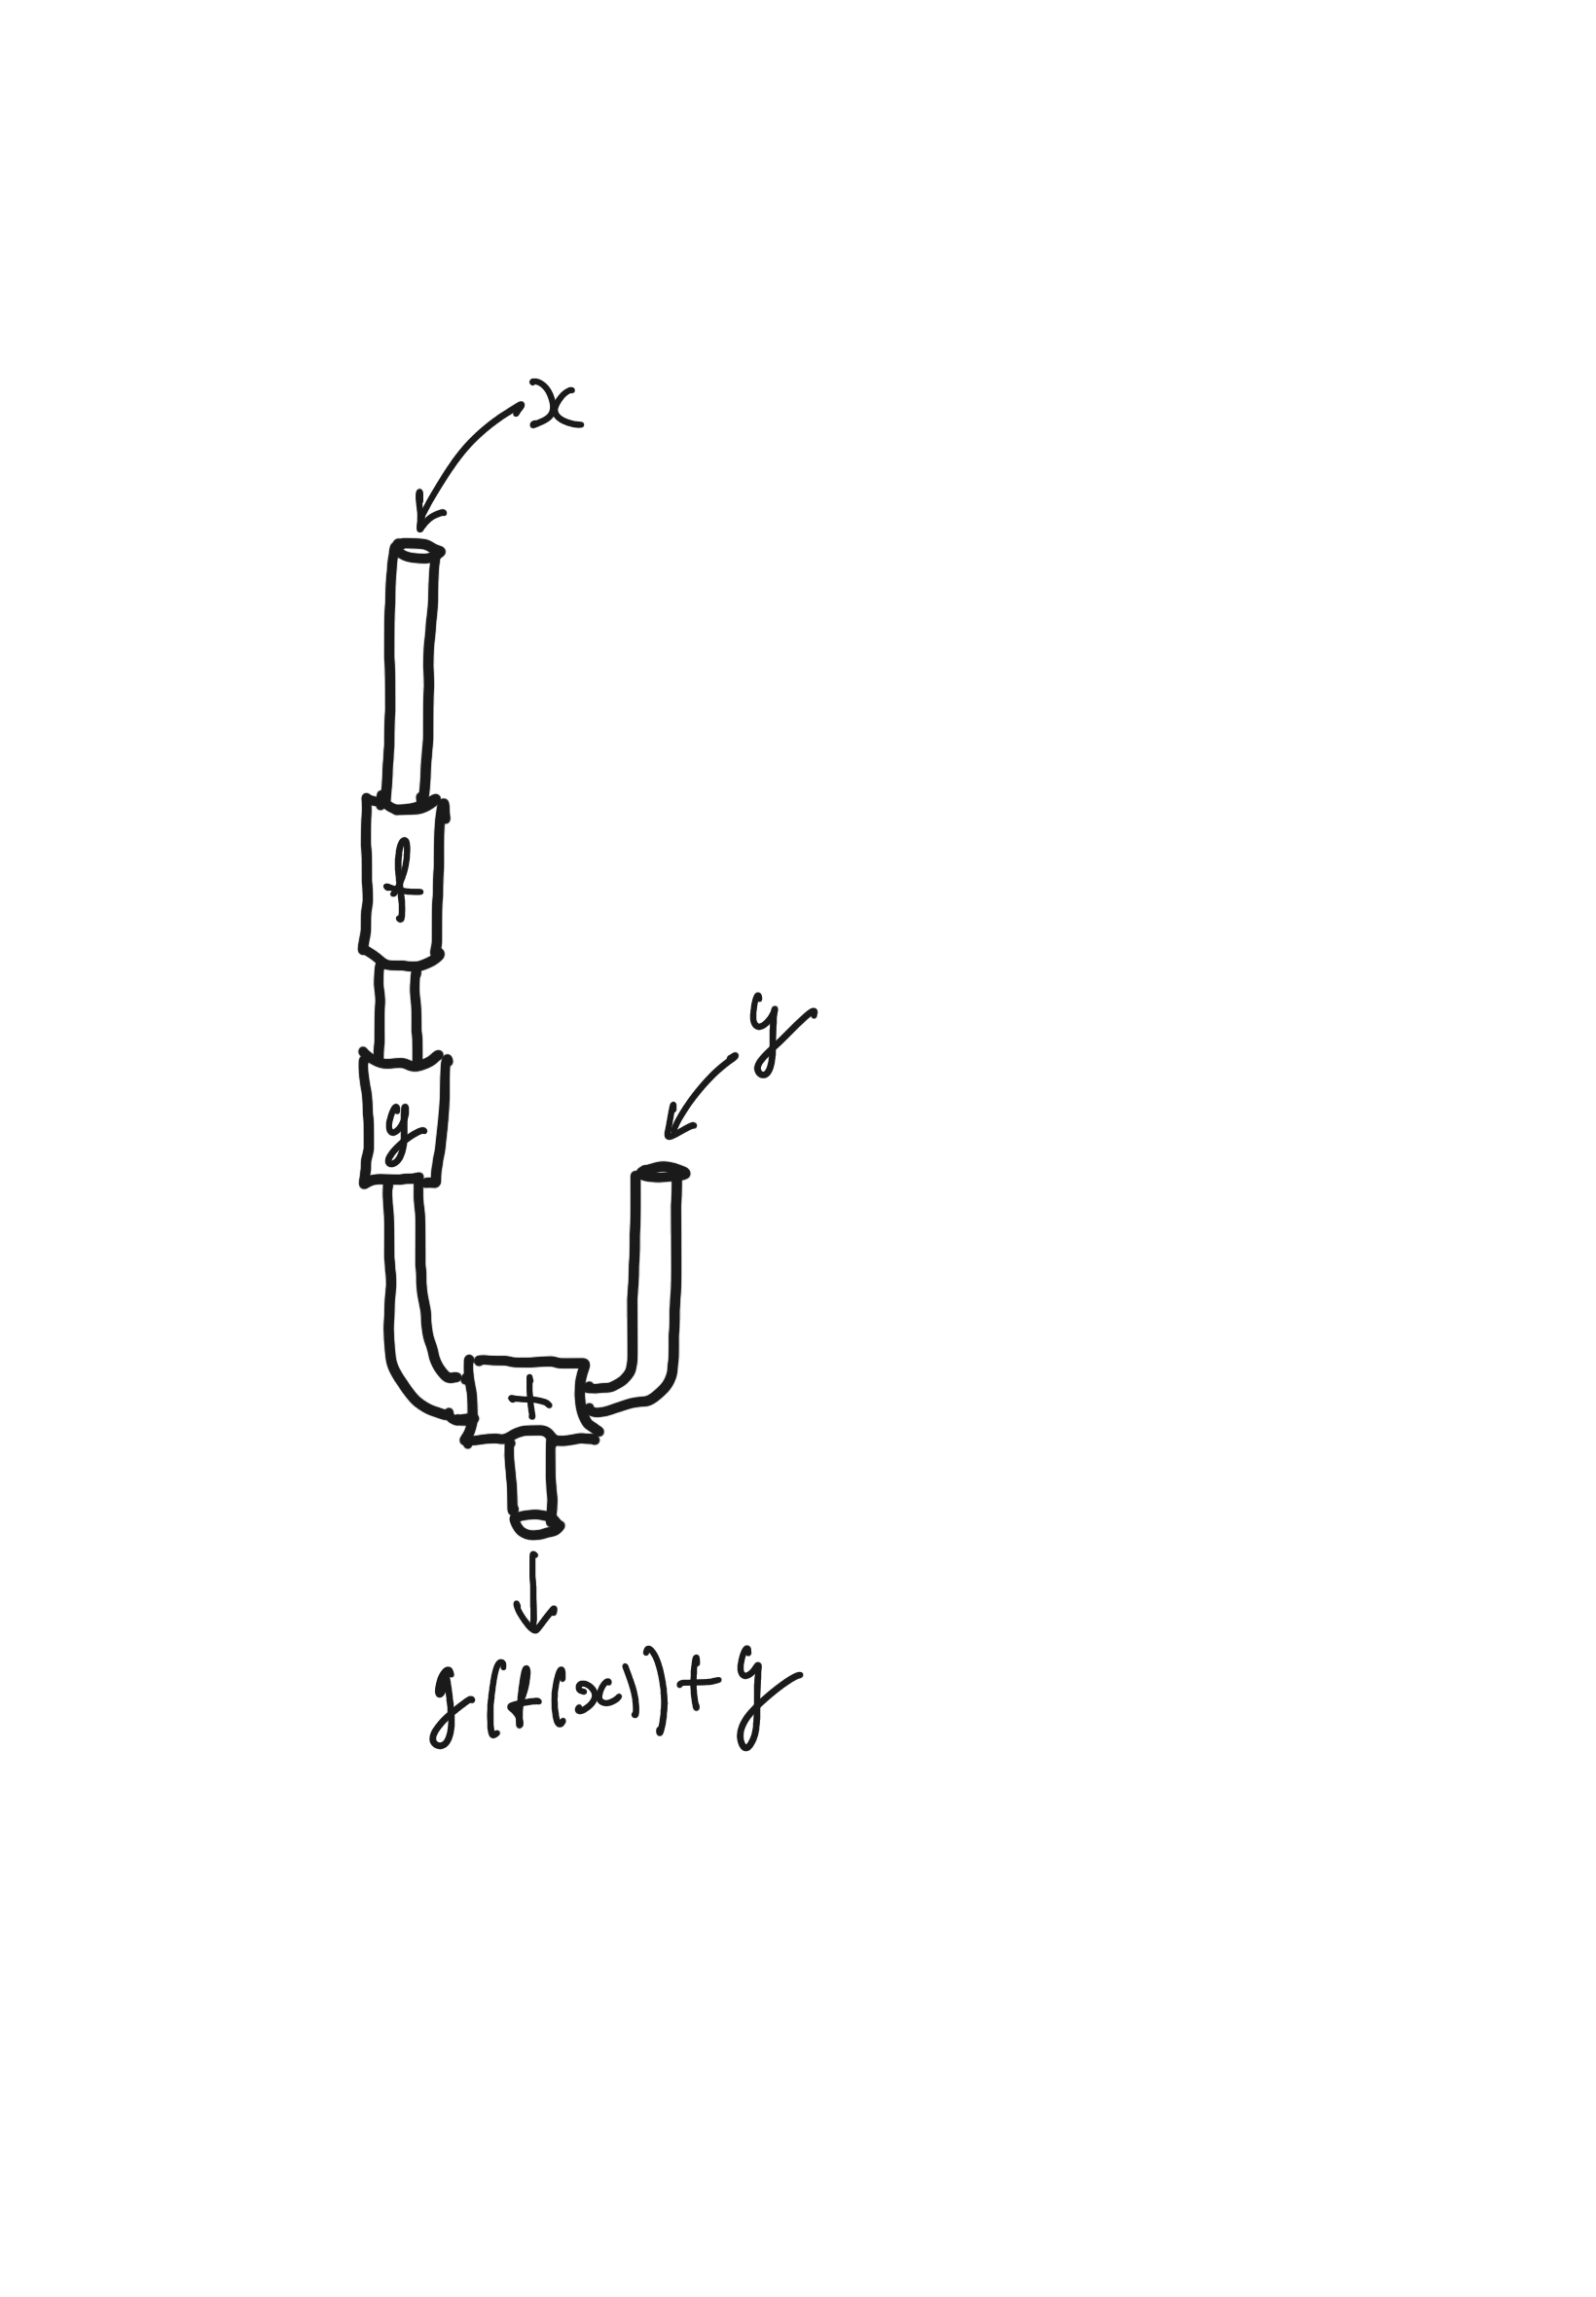
\includegraphics[width=6cm]{images/pipes}
\end{figure}

}

\frame{\frametitle{Сравнение}

\begin{figure}
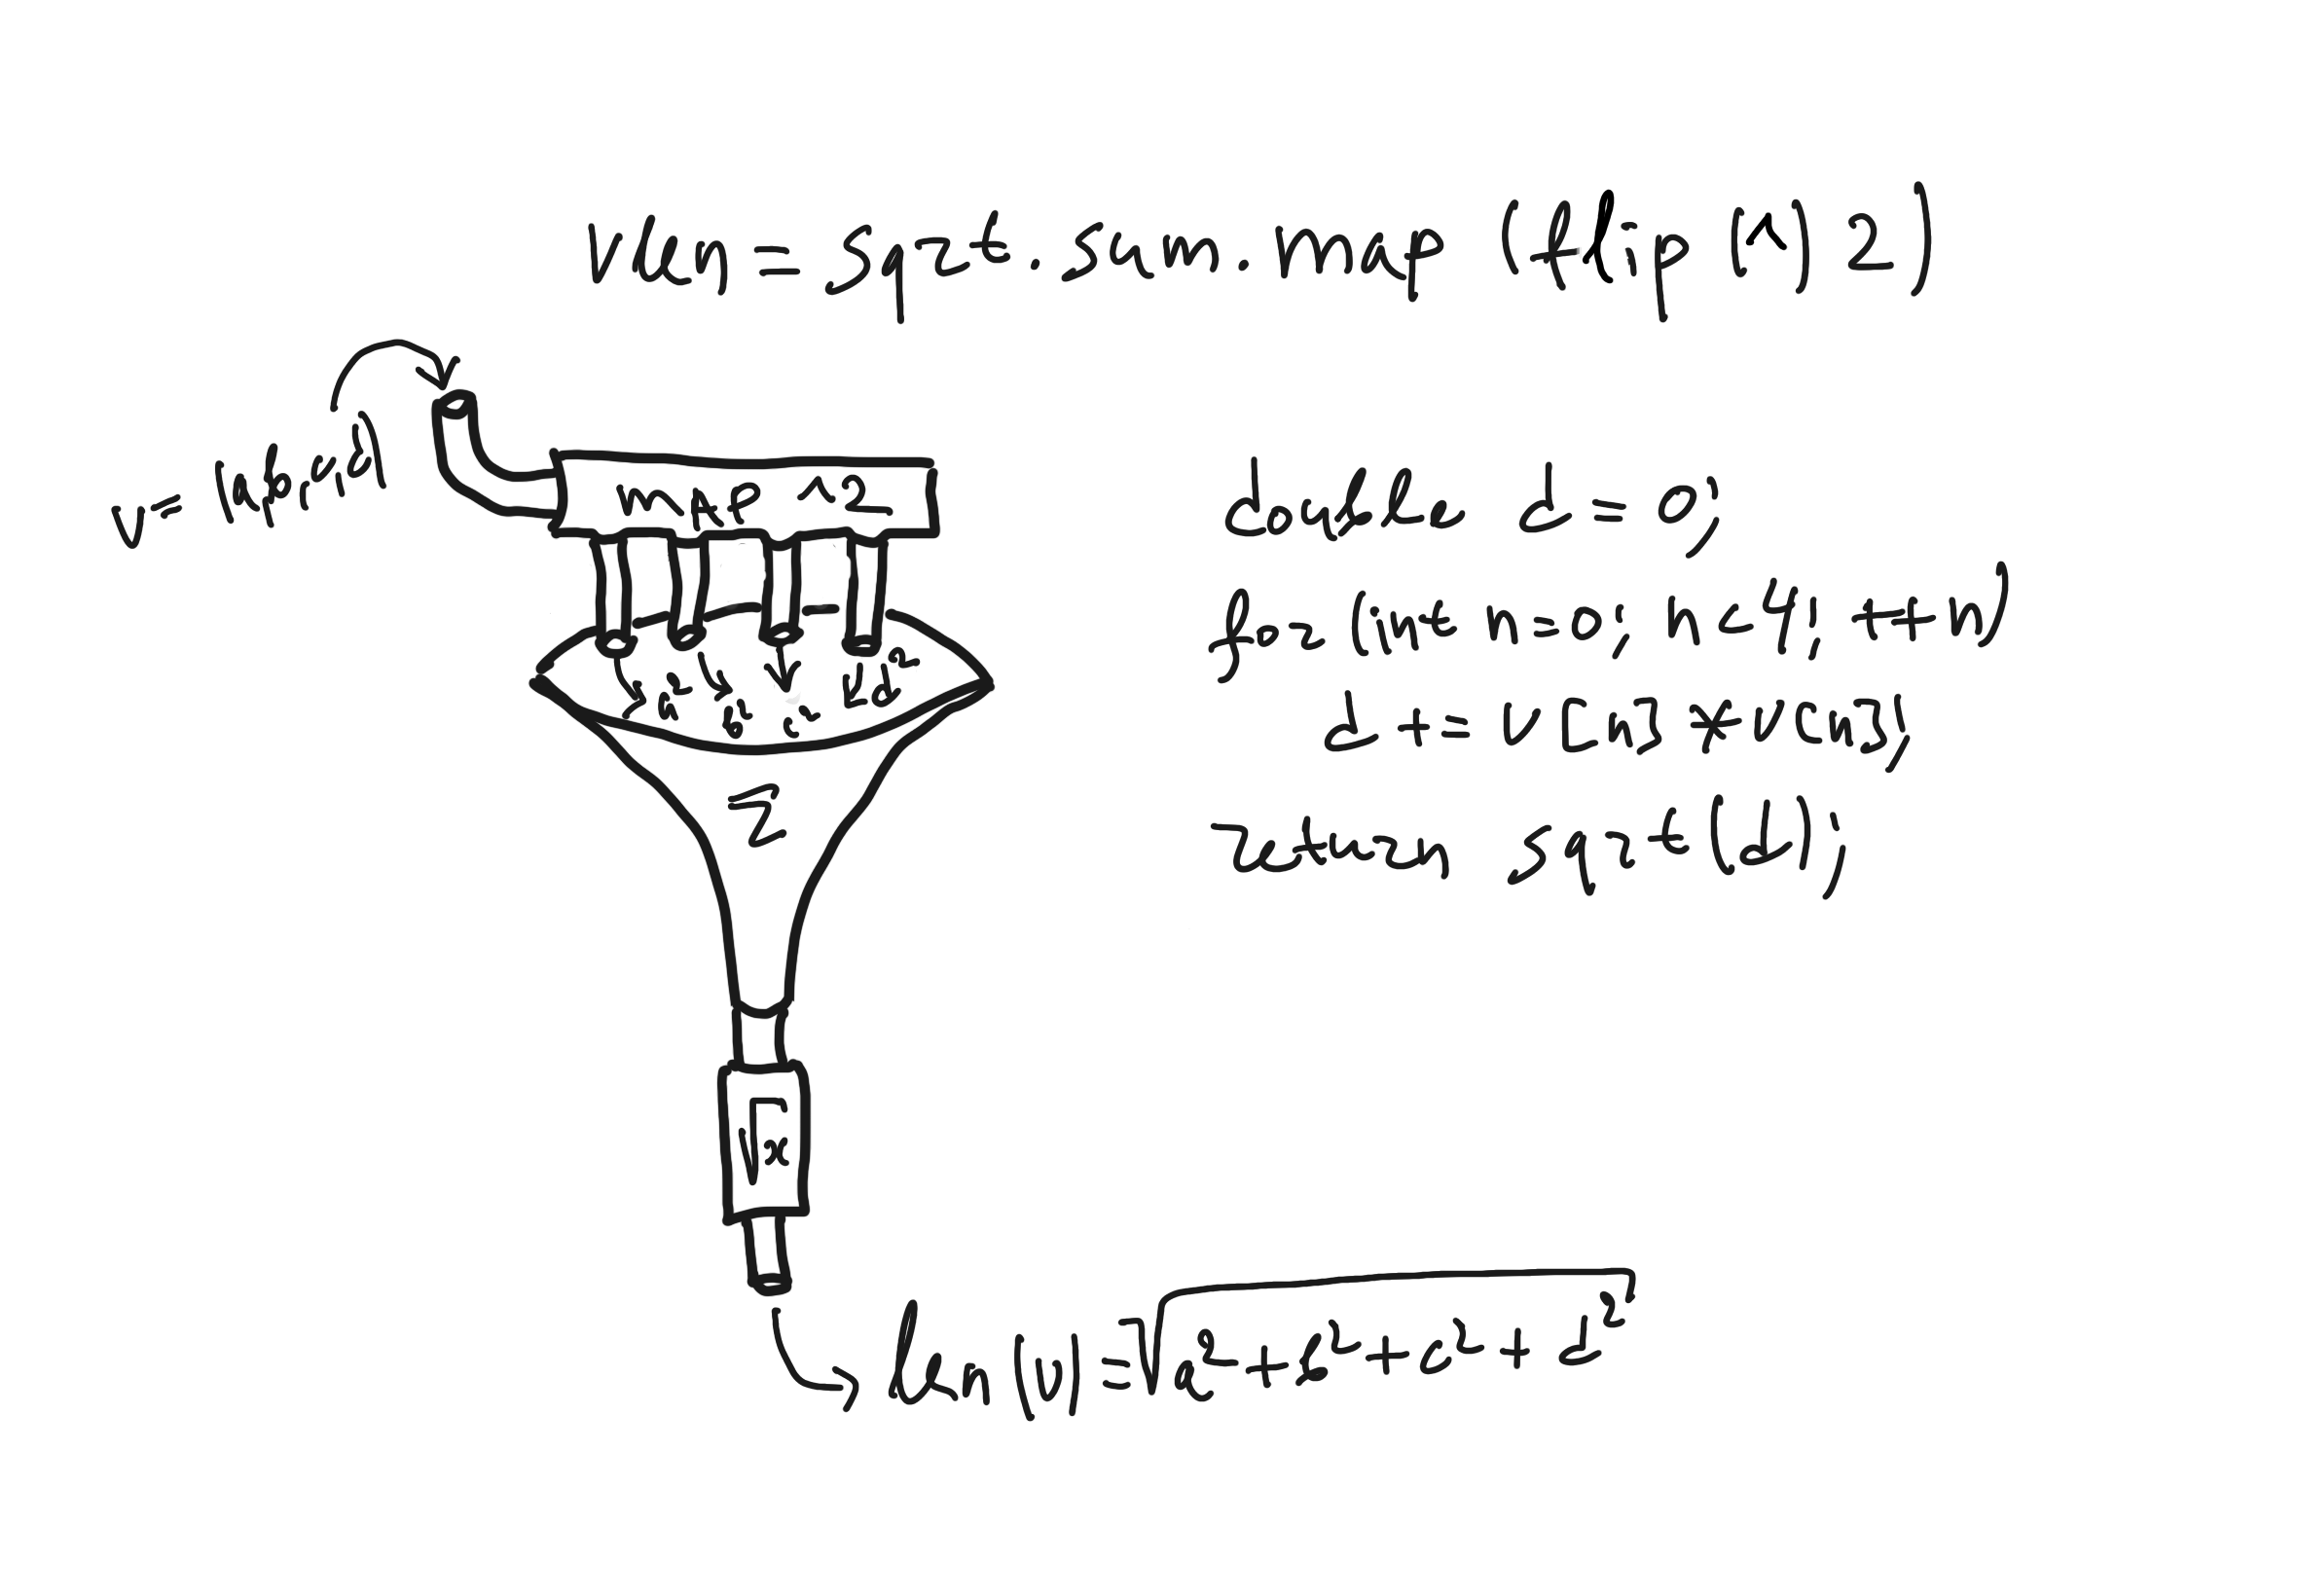
\includegraphics[width=12cm]{images/vlen}
\end{figure}

}



\end{document}



\begin{columns}[t]
  \begin{column}{0.2\textwidth}

\relscale{0.63}
\begin{lstlisting}
\end{lstlisting}
\relscale{1}

  \end{column}
  \begin{column}{0.8\textwidth}

  \end{column}
\end{columns}

#
